\section{Question 1}
This homework used the below equation to simulate the position and velocity of the Hubble space telescope.
\begin{align*}
    \ddot x& - 2n\dot y -3n^2x = f_x \\
    \ddot y& + 2n\dot x = f_y \\
    \ddot z& + n^2z= f_z
\end{align*}
assumed that:
\begin{align*}
    f_x& = 0 \\
    f_y& = 0 \\
    f_z& = 0
\end{align*}
where:
\begin{equation*}
    n = \sqrt{\dfrac{\mu}{r^3}}, \quad \mu = 398600.4418 \text{ km}^3 \text{ s}^{-2}, \quad r = r_{altitude} + r_{earth} = 590 + 6378 = 6968_{km}
\end{equation*}
and initial conditions:
$$
r_{relative} = 
\begin{bmatrix}
    0 & 0 & 0
\end{bmatrix}^{T}, \quad v_{relative} = \begin{bmatrix}
    -0.1 & -0.04 & -0.02
\end{bmatrix}_{m/s}^{T}
$$

\begin{figure}[H]
    \caption{position of the Hubble space telescope}
    \centering
    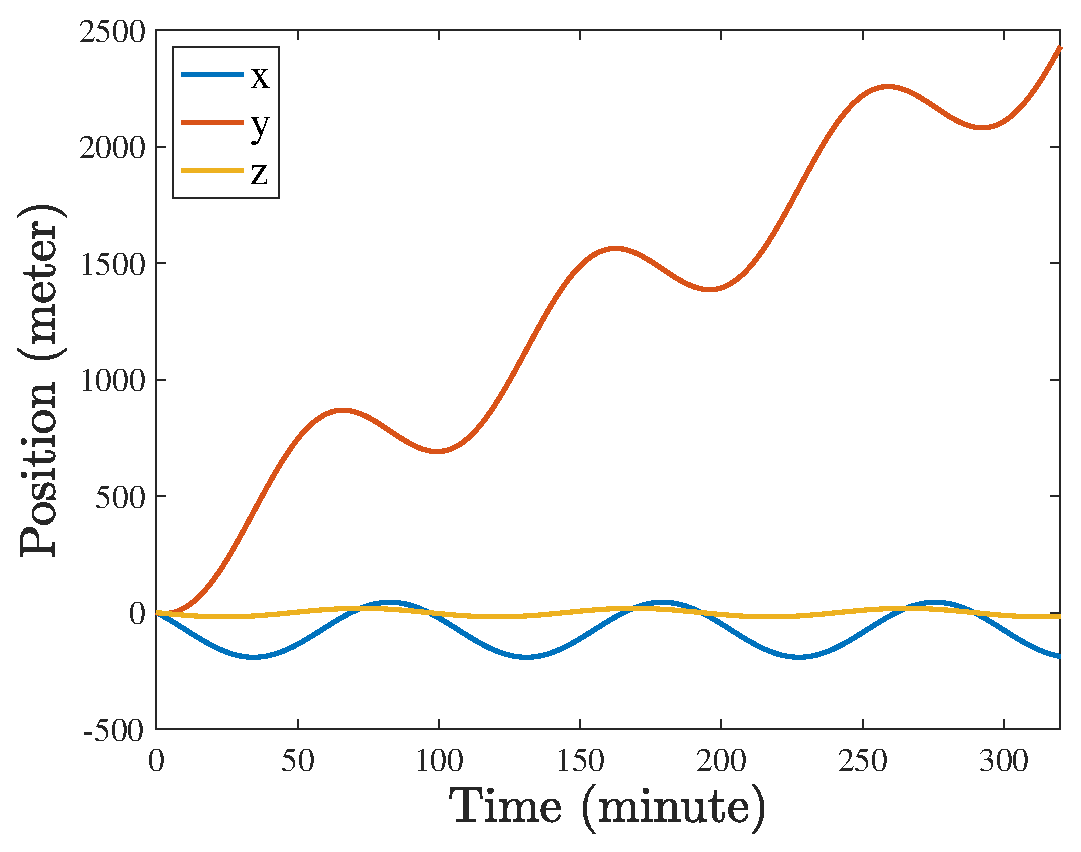
\includegraphics[width=12cm]{../Figure/Q1/position}
\end{figure}

\begin{figure}[H]
    \caption{velocity of the Hubble space telescope}
    \centering
    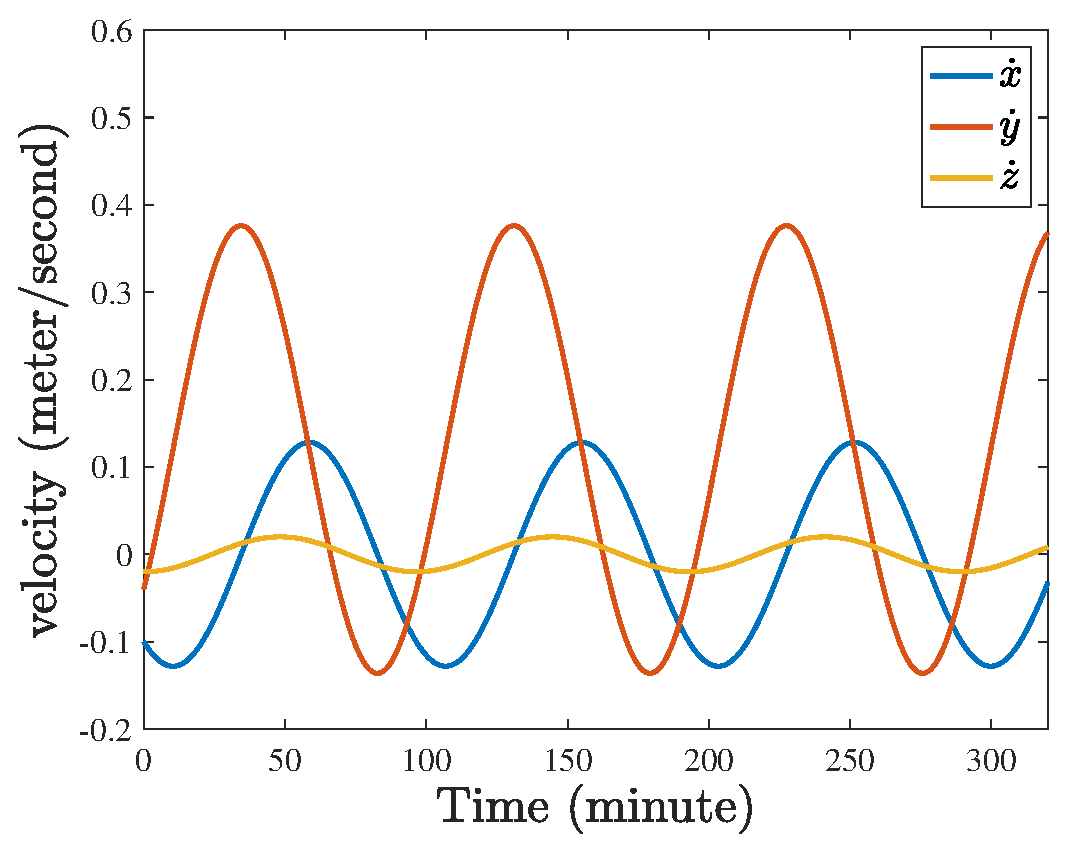
\includegraphics[width=12cm]{../Figure/Q1/velocity}
\end{figure}




